\documentclass[9pt]{extarticle}

\usepackage[utf8]{inputenc}              % Tipos de caracteres
\usepackage[portuguese]{babel}           % Português
\usepackage[a4paper,portrait]{geometry}  % Tipo de papel
\usepackage{color}                       % Para tratamento da cor
\usepackage{graphicx}                    % Para a imagem
\DeclareGraphicsExtensions{.jpg,.png}
\usepackage{amsmath}                     % Para as matematiquices
\usepackage{amssymb}
\usepackage{array}
\usepackage{gensymb}                     % Grau
\usepackage{multicol}
\setlength{\columnsep}{1cm}
\usepackage{geometry}					% Margens
%\usepackage{xfrac}
\usepackage{colortbl}

\usepackage{multirow}

\addtolength{\topmargin}{-25mm}
\addtolength{\textheight}{60mm}
\addtolength{\oddsidemargin}{-23mm}
\addtolength{\textwidth}{48mm}

\renewenvironment{abstract}
 {\small
  \begin{center}
  \bfseries \abstractname\vspace{-.5em}\vspace{0pt}
  \end{center}
  \list{}{
    \setlength{\leftmargin}{0cm}%
    \setlength{\rightmargin}{\leftmargin}%
  }%
  \item\relax}
 {\endlist}
 
\renewcommand{\abstractname}{Resumo}

\delimitershortfall-1sp
\newcommand\abs[1]{\left|#1\right|}
\newcommand{\PR}[1]{\ensuremath{\left[#1\right]}}
\newcommand{\PC}[1]{\ensuremath{\left(#1\right)}}
\newcommand{\chav}[1]{\ensuremath{\left\{#1\right\}}}

\newcolumntype{x}[1]{>{\centering\hspace{0pt}}p{#1}}

\begin{document}

\title {\bf \huge Estudo de Transformações Adiabáticas e Isotérmicas do Ar}
\author
{{\small João Ferreira (78179) Henrique Rodrigues (78632) Rodrigo C. Carvalho (78646) Cristina Melício (78947)} \\
{\small MEFT $\cdot$ 2ºAno, 2º Semestre $\cdot$ Laboratório de Complementos de Eletromagnetismo e Termodinâmica}}
\date{{\small Grupo III $\cdot$ Sexta-Feira $\cdot$ 20 de Março de 2015}}
\maketitle

\begin{abstract}
\par Nesta experiência estudaram-se fenómenos de compressão e expansão adiabáticas e isotérmicas. Obtiveram-se os valores para o expoente experimental $\alpha=1.400\pm0.002$ e $\alpha=1.405\pm0.005$ para os casos adiabáticos e  $\alpha=1.015\pm0.003$ e $\alpha=1.05\pm0.02$ para os isotérmicos, referentes à relação $PV^{\alpha}=const$
\end{abstract}

\begin{multicols}{2}

\section{Introdução}

\par Neste trabalho será explorado o comportamento de ar dentro de uma campânula quando sujeito a expansões e compressões adiabáticas e isotérmicas, sendo este considerado para efeitos do seu estudo um gás ideal. De facto, o modelo do gás ideal consiste em assumir as partículas de um dado gás como pontuais e desprovidas de interacções entre si, movendo-se aleatoriamente e cujas colisões são elásticas - notando-se desde já, consequentemente, que toda a energia do gás é cinética. A lei que codifica este modelo teórico designa-se Lei dos Gases Perfeitos, dada pela seguinte expressão:
\begin{equation} \label{perfeitos}
PV = nRT
\end{equation}
\begin{center}
\par\noindent {\scriptsize(em que $P$ é a pressão, $V$ o volume, $n$ o número de moles, $R$ a constante dos gases perfeitos e $T$ a temperatura do gás)}
\end{center}

\par É de notar que, para o ar atmosférico em condiçoes PTN ou perto delas, o modelo revela-se compatível. Visto as condições de realização da experiência não destoarem em demasia em relação a estas pode-se depreender que a utilização deste modelo será válida.

\par De acordo com a Primeira Lei da Termodinâmica, considerando um dado sistema fechado, a variação infinitesimal de energia desse sistema pode ser dada pela seguinte relação:
\begin{equation}
dU = \delta Q - \delta W 
\end{equation}
\begin{center}
\par\noindent {\scriptsize(em que $dU$ é a variação infinitesimal da energia interna, $\delta Q$ o calor infinitesimal que o sistema recebe e $\delta W$ o trabalho infinitesimal que o sistema fornece ao exterior)}
\end{center}
\par Sabe-se ainda que para os gases ideias a energia interna é apenas função da temperatura. Sendo assim, tem-se que a variação da energia interna e do trabalho podem ser descritos pelas equações:
\begin{eqnarray} \label{dU} 
dU &=& n C_V dT \\
\delta W &=& P dV  
\end{eqnarray}
\par O ar atmosférico que será estudado pode ser considerado aproximadamente um gás diatómico ideal, sendo assim a capacidade térmica a volume constante $C_V = \frac{5}{2} R$ e a pressão constante é $C_P = \frac{7}{2} R$.
\par Tem-se ainda a relação entre estas duas grandezas dada por:
\begin{equation}
\gamma = \frac{C_P}{C_V} = 1,4
\end{equation}

\subsection*{Transformação adiabática}

\par Uma transformação adiabática é um processo em que não existem trocas de calor com o exterior, ou seja, $\delta Q = 0$, aplicando a expressão (2):
\begin{equation} \label{adia}
dU = -\delta W 
\end{equation}
\par Tem-se a seguinte igualdade para uma transformação ideal reversível, em que a variação de entropia é nula e realizada quase-estaticamente: 
\begin{equation} \label{alpha}
PV^{\gamma} = const
\end{equation}

\par Sendo assim, da integração de ambos os membros da expressão \eqref{adia} tem-se que: 
\begin{equation}
\Delta U = n C_v \Delta T = \frac{P_fV_f-P_iV_i}{1-\gamma} = W
\end{equation}
\par Notemos que outra forma de determinar o valor do trabalho é, obviamente, através da integração numérica do diagrama $P(V)$.

\subsection*{Transformação isotérmica}

\par Uma transformação isotérmica é um processo em que a temperatura se mantém constante. Como a energia interna depende apenas da temperatura tem-se então, naturalmente, que $d U = 0$ e $PV=const$. Aplicando a expressão (2):
\begin{equation}
\delta Q = \delta W 
\end{equation}
\par Assim, facilmente se depreende que:
\begin{equation}
Q = W = nRT \ln \left(\frac{V_f}{V_i} \right)
\end{equation}
\par Alternativamente, tal como no caso adiabático, o trabalho pode ainda ser calculado por integração numérica da curva $P(V)$.

\subsection*{Correções}

\par Os casos acima expostos correspondem, naturalmente, a processos ideais. No entanto, existem modelos mais gerais para o estudo de compressões e expansões adiabáticas com trocas de calor. Existe a necessidade de os definir uma vez que cada um dos processos apresentados anteriormente não ocorre de forma ideal. Para uma transformação adiabática haverá sempre, em termos práticos, uma troca de calor, ou seja $\delta Q \neq 0$ e para uma transformação isotérmica experimental a temperatura não se mantém constante ou seja $dU \neq 0$. 

\par Seja $\alpha$ o expoente obtido experimentalmente para o volume em $PV^{\alpha}$. Temos pela lei (2) que:
\begin{equation}
\delta Q = nRdT + \frac{nR}{1-\alpha}dT = n \left(C_V + \frac{R}{1-\alpha}\right) dT
\end{equation}

\par Sendo assim, o calor transferido esperado, para cada processo, em função do parâmetro $\alpha$ é  dado pela seguinte expressão:
\begin{equation} \label{Q}
Q = n \left(C_V + \frac{R}{1-\alpha}\right) \Delta T
\end{equation} 

\section{Montagem da Experiência}

\par A montagem associada a esta experiência é formada por um dispositivo de compressão/expansão constituído por um cilindro graduado, um pistão que é movido pelo utilizador através de um braço relativamente extenso, duas torneiras na parte inferior do cilindro que permitem controlar o fluxo de ar que entra ou sai deste. Na montagem existem também duas fontes de tensão responsáveis por alimentar os sensores e pré-amplificadores eletrónicos, e um computador no qual se corre o software \textit{Data Monitor} responsável pela aquisição e tratamento dos dados. Para recolher as informações relativamente à pressão e temperatura do gás foram utilizados dois transcondutores, o de pressão - um sensor piezzo-resistivo- e o de temperatura - um fino fio de níquel com elevada resistividade térmica -, montados na base do cilindro. 

\par O diagrama da montagem encontra-se representado na figura 1.

%\vspace{-0.5cm}
\hspace{-0.8cm}
\begin{center}
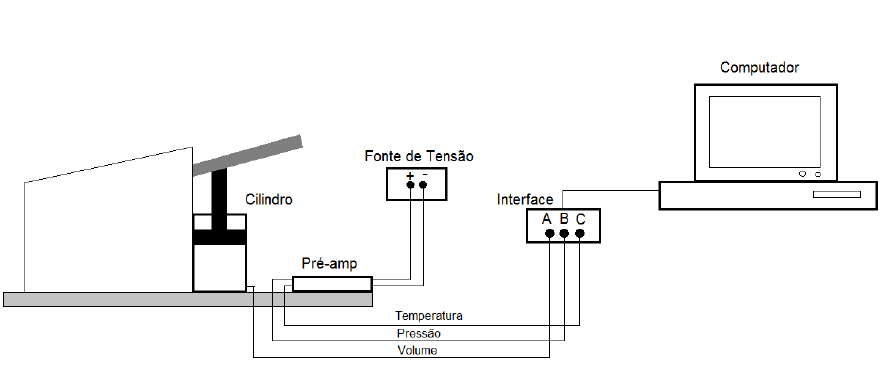
\includegraphics[width=260pt]{diagrama.png}
\begin{center}
\par\noindent {\scriptsize ({\bf Figura 1}: Diagrama da experiência)}
\end{center}
\end{center}

\section{Dados Experimentais}

\subsection*{Calibração}

\par Começou-se por calibrar o sensor de volume. Para tal, mediu-se para diferentes valores de tensao, o valor da altura $h$ do pistão indicada no cilindro. O volume será dado por:
\begin{equation}
V = \pi\PC{\frac{d}{2}}^2\PC{h+0.06}
\end{equation}
\begin{center}
\par\noindent {\scriptsize (Onde $d=4.409cm$ é o diâmetro do tubo)}
\end{center}

\subsection*{Compressão Adiabática}

\par Após colocar o pistão na posição de volume máximo e fechar as torneiras que tinham sido mantidas abetas para equilibrar a pressão e a temperatura do gás, com o programa \verb|DM| no modo {\it osciloscope} com a base de tempos em $10ms$ por divisão, comprimiu-se rapidamente o gás, de modo a evitar trocas de calor. Os dados foram registados e foi-lhes aplicado o logaritmo, representando-se no seguinte gráfico os pontos de $\log{P}$ como função de $\log{V}$, aos quais se ajustou uma equação do tipo:

\begin{equation} \label{LADB1}
\log{P}\PC{\log{V}}=c_1-\alpha\log{V}
\end{equation}

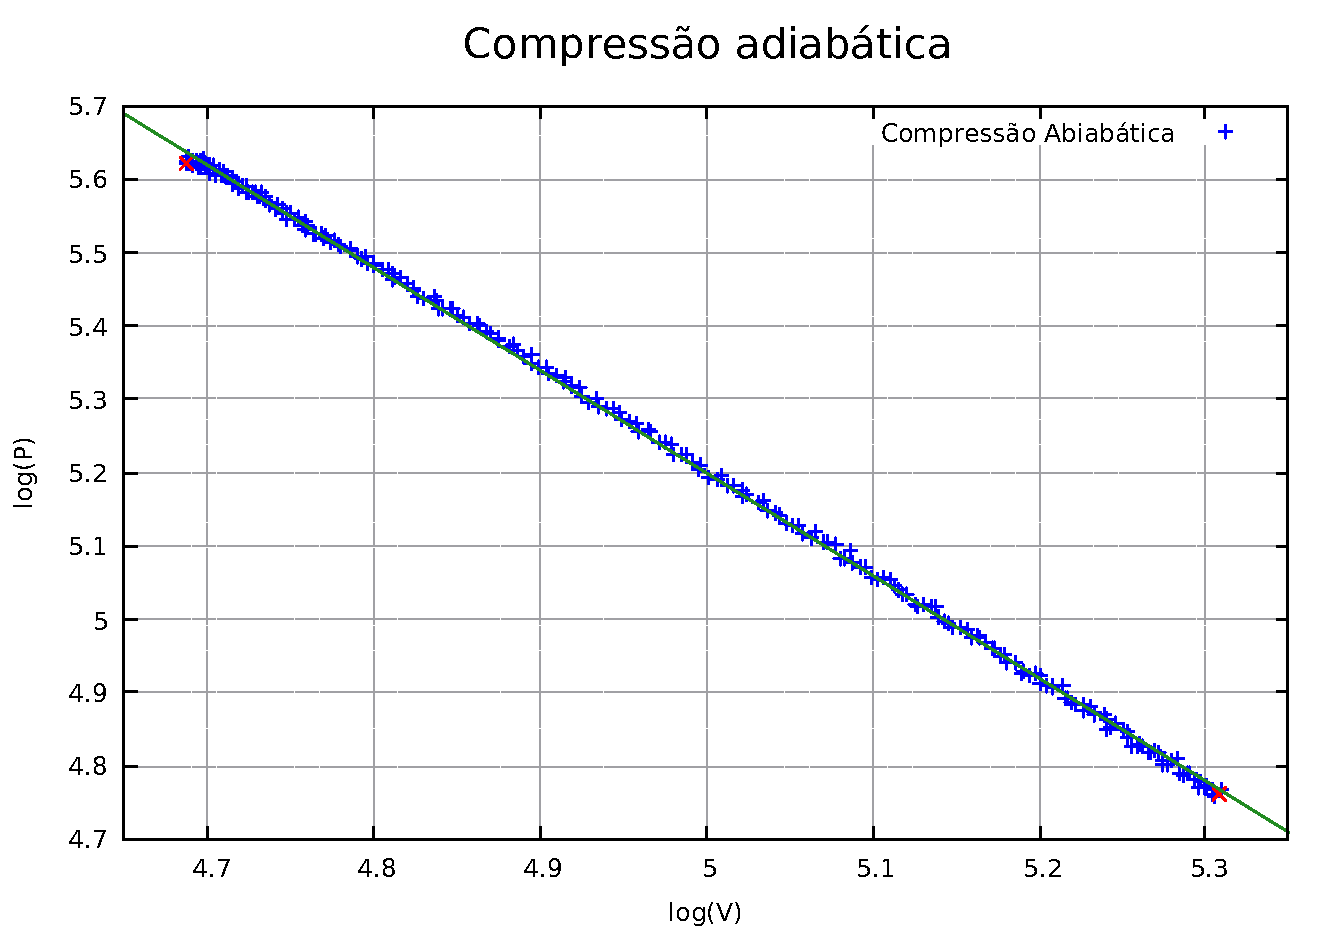
\includegraphics[width=220pt]{LADB1.pdf}
\begin{center}
\par\noindent {\scriptsize ({\bf Gráfico 1}: Valores do logaritmo da pressão como função do logaritmo do volume, para uma compressão adiabática. A verde representa-se o ajuste da equação \eqref{LADB1} obtido pelo método dos mínimos quadrados. A vermelho indicam-se os pontos $(4.69,5.62)$ e $(5.31,4.76)$, da esquerda para a direita)}
\end{center}

\par Obtiveram-se os seguintes parâmetros \footnote{O valor retornado pelo programa {\it Gnuplot} para $\alpha$ e utilizado nos posteriores cálculos foi 1.40036}:

\begin{center}
\begin{tabular}{ x{1cm} x{2.5cm} }
\hline \hline
$\alpha$ & 1.400$\pm$0.002 \tabularnewline
$c_1$ & 12.20$\pm$0.01 \tabularnewline
\hline \hline
\end{tabular}
\end{center}

\par Por último, analisou-se o balanço energético da compressão. A variação da energia interna $\Delta U$, é dada pela integração da expressão \eqref{dU}, o trabalho realizado pelo pistão calculado numericamente usando o programa \verb|DM|, e o calor esperado $Q_0$ é dado por \eqref{Q}. De modo a poder efetuar estes cálculos, é também necessário conhecer o valor da variação da temperatura $\Delta T$ e do número de moles de gás $n$. Para $\Delta T$, fez-se a diferença entre as médias das temperaturas dos cinco primeiros e dos cinco últimos valores recolhidos. Para $n$ utilizou-se a expressão \eqref{perfeitos} e fez-se a média entre os cinco primeiros valores. Obtiveram-se os seguintes resultados: \footnote{Considerou-se a constante dos gases perfeitos $R=8.314462$.}

\begin{center}
\begin{tabular}{ x{2cm} x{3cm} }
\hline \hline
$\Delta T$ $(K)$ & 83$\pm$3 \tabularnewline
$n$ $(mol)$ & (9.48$\pm$0.02)$\times10^{-3}$ \tabularnewline
$\Delta U$ $(J)$ & 16.34$\pm$0.07 \tabularnewline
$W$ $(J)$ & 16.5$\pm$0.2 \tabularnewline
$Q$ $(J)$ & -0.2$\pm$0.3 \tabularnewline
$Q_0$ $(J)$ & 0.01$\pm$0.08 \tabularnewline
\hline \hline
\end{tabular}
\end{center}

\subsection*{Compressão Isotérmica}

\par Repetiu-se o procedimento anterior, mas colocou-se a base de tempos em 100 ms por divisão. Comprimiu-se lentamente o pistão enquanto se verificava no écran que a linha correspondente à temperatura se mantinha constante. Os dados foram registados e foi-lhes aplicado o logaritmo, representando-se no seguinte gráfico os pontos de $\log{P}$ como função de $\log{V}$, aos quais se ajustou uma equação do tipo \eqref{LADB1}:

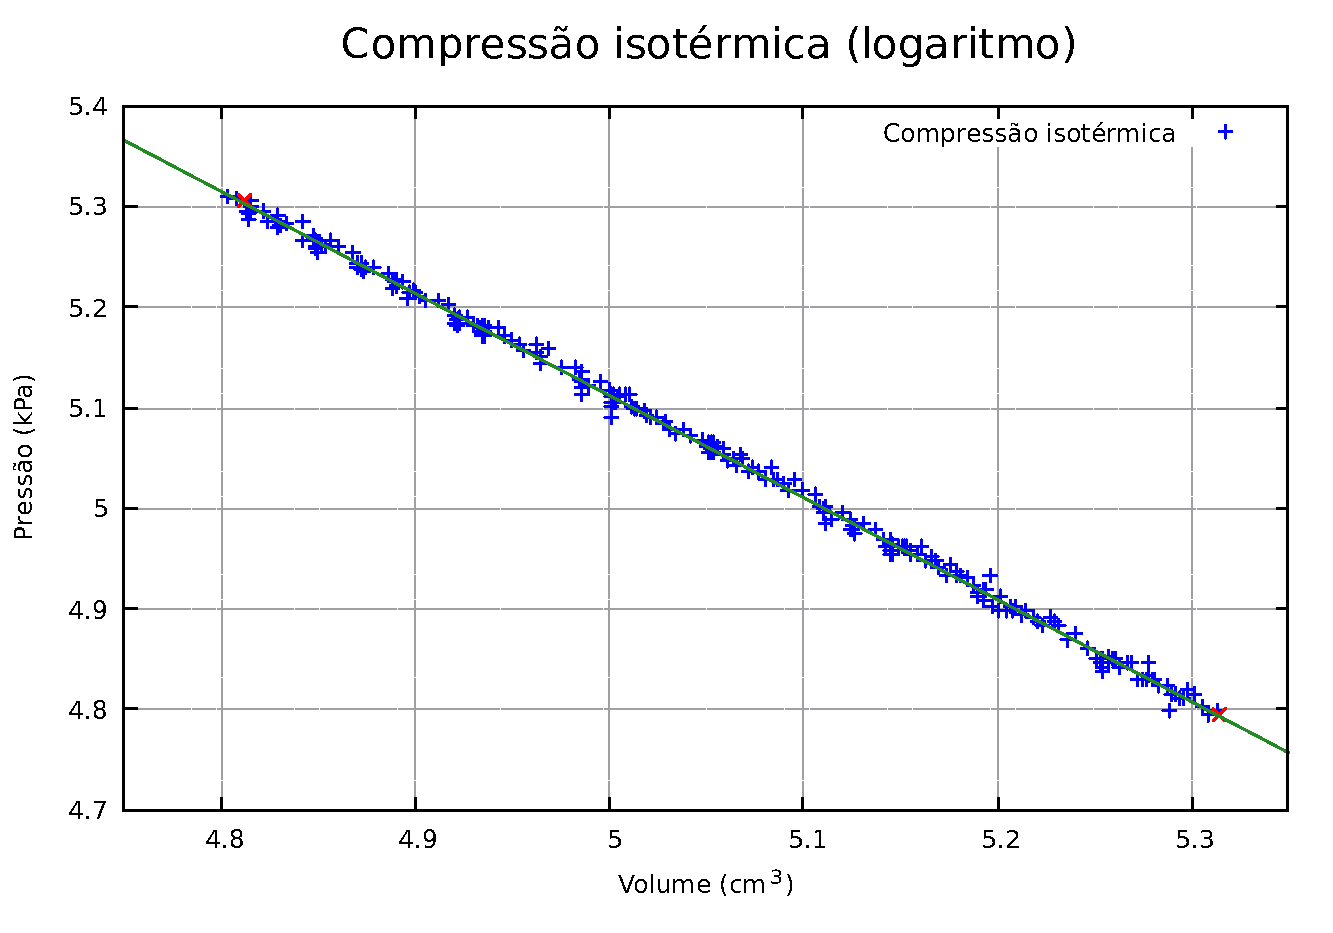
\includegraphics[width=220pt]{lcomp_iso.pdf}
\begin{center}
\par\noindent {\scriptsize ({\bf Gráfico 2}: Valores do logaritmo da pressão como função do logaritmo do volume, para uma compressão isotérmica. A verde representa-se o ajuste da equação \eqref{LADB1} obtido pelo método dos mínimos quadrados. A vermelho indicam-se os pontos $(4.81,5.31)$ e $(5.31,4.79)$, da esquerda para a direita)}
\end{center}

\par Obtiveram-se os seguintes parâmetros:

\begin{center}
\begin{tabular}{ x{1cm} x{2.5cm} }
\hline \hline
$\alpha$ & 1.015$\pm$0.003 \tabularnewline
$c_1$ & 10.19$\pm$0.02 \tabularnewline
\hline \hline
\end{tabular}
\end{center}

\par Quanto ao balanço energético da compressão, obtiveram-se os seguintes resultados:

\begin{center}
\begin{tabular}{ x{2cm} x{3cm} }
\hline \hline
$\Delta T$ $(K)$ & 0.9$\pm$2.9 \tabularnewline
$n$ $(mol)$ & (9.70$\pm$0.02)$\times10^{-3}$ \tabularnewline
$\Delta U$ $(J)$ & 0.2$\pm$0.6 \tabularnewline
$W$ $(J)$ & 12.6$\pm$0.2 \tabularnewline
$Q$ $(J)$ &-12.4$\pm$0.8 \tabularnewline
$Q_0$ $(J)$ & -5$\pm$16 \tabularnewline
\hline \hline
\end{tabular}
\end{center}

\subsection*{Expansão Adiabática}

\par Repetiu-se o primeiro procedimento, mas colocou-se o pistão na posição de volume mínimo. Expandiu-se rapidamente o gás de modo a evitar trocas de calor. Os dados foram registados no programa \verb|DM| e foi-lhes aplicado o logaritmo, representando-se no seguinte gráfico os pontos de $\log{P}$ como função de $\log{V}$, aos quais se ajustou uma equação do tipo \eqref{LADB1}:

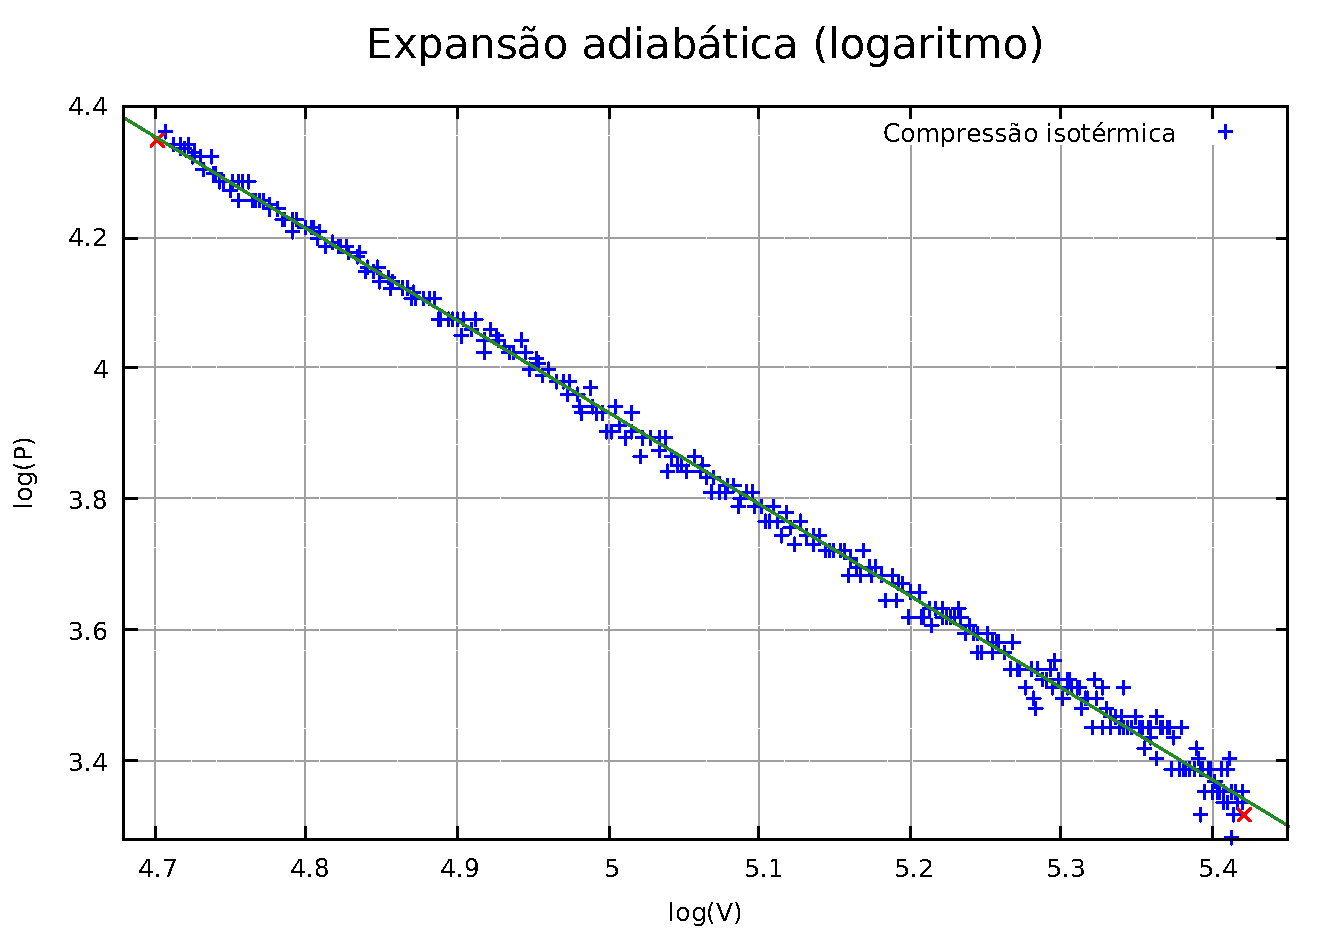
\includegraphics[width=220pt]{lexp-adb.pdf}
\begin{center}
\par\noindent {\scriptsize ({\bf Gráfico 3}: Valores do logaritmo da pressão como função do logaritmo do volume, para uma compressão isotérmica. A verde representa-se o ajuste da equação \eqref{LADB1} obtido pelo método dos mínimos quadrados. A vermelho indicam-se os pontos $(4.70,4.35)$ e $(5.42,3.32)$, da esquerda para a direita)}
\end{center}

\par Obtiveram-se os seguintes parâmetros:

\begin{center}
\begin{tabular}{ x{1cm} x{2.5cm} }
\hline \hline
$\alpha$ & 1.405$\pm$0.005 \tabularnewline
$c_1$ & 10.96$\pm$0.03 \tabularnewline
\hline \hline
\end{tabular}
\end{center}

\par Quanto ao balanço energético da expansão, obtiveram-se os seguintes resultados:

\begin{center}
\begin{tabular}{ x{2cm} x{3cm} }
\hline \hline
$\Delta T$ $(K)$ & -75$\pm$14 \tabularnewline
$n$ $(mol)$ & (3.58$\pm$0.03)$\times10^{-3}$ \tabularnewline
$\Delta U$ $(J)$ & -5.6$\pm$0.9 \tabularnewline
$W$ $(J)$ & 5.3$\pm$0.2 \tabularnewline
$Q$ $(J)$ & -0.2$\pm$1.2 \tabularnewline
$Q_0$ $(J)$ & -0.07$\pm$0.08 \tabularnewline
\hline \hline
\end{tabular}
\end{center}

\par De notar a formação de uma espécie de nuvem branca, no centro do cilindro.

\subsection*{Expansão Isotérmica}

\par Repetiu-se o segundo procedimento, mas colocou-se o pistão na posição de volume mínimo. Expandiu-se lentamente o gás de modo a evitar variação de temperatura. Os dados foram registados no programa \verb|DM| e foi-lhes aplicado o logaritmo, representando-se no seguinte gráfico os pontos de $\log{P}$ como função de $\log{V}$, aos quais se ajustou uma equação do tipo \eqref{LADB1}:

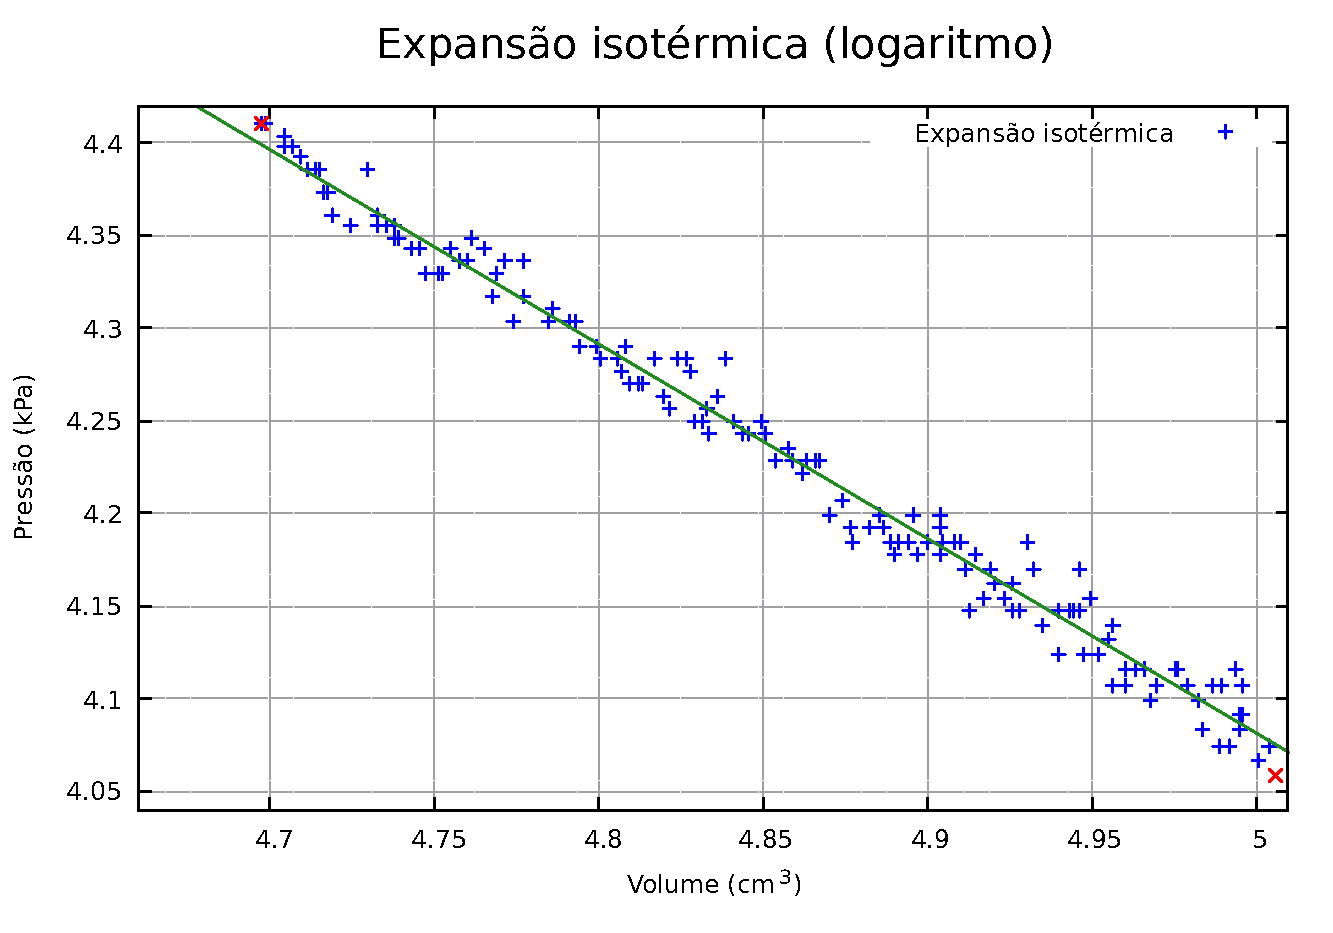
\includegraphics[width=220pt]{lexp_iso.pdf}
\begin{center}
\par\noindent {\scriptsize ({\bf Gráfico 4}: Valores do logaritmo da pressão como função do logaritmo do volume, para uma compressão isotérmica. A verde representa-se o ajuste da equação \eqref{LADB1} obtido pelo método dos mínimos quadrados. A vermelho indicam-se os pontos $(4.70,4.41)$ e $(5.01,4.06)$, da esquerda para a direita)}
\end{center}

\par Obtiveram-se os seguintes parâmetros:

\begin{center}
\begin{tabular}{ x{1cm} x{2.5cm} }
\hline \hline
$\alpha$ & 1.05$\pm$0.02 \tabularnewline
$c_1$ & 9.33$\pm$0.06 \tabularnewline
\hline \hline
\end{tabular}
\end{center}

\par Quanto ao balanço energético da expansão, obtiveram-se os seguintes resultados:

\begin{center}
\begin{tabular}{ x{2cm} x{3cm} }
\hline \hline
$\Delta T$ $(K)$ & -7$\pm$7 \tabularnewline
$n$ $(mol)$ & (3.81$\pm$0.01)$\times10^{-3}$ \tabularnewline
$\Delta U$ $(J)$ & -0.5$\pm$0.5 \tabularnewline
$W$ $(J)$ & 2.7$\pm$0.2 \tabularnewline
$Q$ $(J)$ & -3.3$\pm$0.7 \tabularnewline
$Q_0$ $(J)$ & 3$\pm$5 \tabularnewline
\hline \hline
\end{tabular}
\end{center}

\par De notar a formação de uma espécie de nuvem branca, no centro do cilindro.

\section{Discussão de Resultados}

\par Após a realização da experiência foi possível extrair diversas conclusões.

\par Relativamente à compressão adiabática, verificou-se que se obteve para a constante experimental o valor $\alpha=1.40036\pm0.002$, possuíndo por conseguinte um desvio à exactidão de $0.03\%$ e um desvio à precisão de $0.14\%$. Isto implica, naturalmente, que o processo de compressão levado a cabo foi quase perfeitamente adiabático. De facto, verificou-se que o calor libertado pelo sistema possui o valor de $Q=(-0.2\pm0.3)J$, podendo ser congruentemente zero dentro da margem de incerteza experimental permitida, tal como esperado. Além disto, por integração da curva P(V) obteve-se um valor para o trabalho de $W=(16.5\pm0.2)J$, enquanto que a variação da energia interna do sistema se obteve como sendo $\Delta U=(16.34\pm0.07)J$. Assim, verificamos que a diferença entre o trabalho e a variação da energia interna pode ser 0 dentro da margem de incerteza permitida pelos respectivos erros, corroborando a hipótese de uma compressão adiabática perfeita implicada pelo valor de $\alpha$ obtido. Como tal, podemos concluir que a aproximação teórica efectuada do ar atmosférico enquanto gás perfeito se revelou perfeitamente adequada para este caso. Notamos ainda que o valor do calor previsto é igualmente 0 dentro da incerteza.

\par Subsequentemente procedeu-se ao estudo de uma compressão isotérmica. Sabemos que para este processo, o valor de $\alpha$ teoricamente previsto corresponde a $1$. Obteve-se experimentalmente para este um valor de $\alpha=1.015\pm0.001$, existindo então um desvio à exactidão de $1,5\%$ e um desvio à precisão de $0.1\%$. Seria expectável, mediante a análise dos valores experimentais da temperatura, que tal ocorresse, visto a variação da temperatura do início para o fim da experiência ser de $\Delta T=(0.9\pm2.9)K$, e por conseguinte congruentemente nula. De facto, o valor de $\alpha$ é 1 dentro da margem de incerteza, e coaduna-se com as previsões teóricas efectuadas. Aliás, verificou-se que a esta variação de temperatura estava associado um valor de variação de energia interna $\DeltaU=(0.2\pm0.6)$J, com um valor de calor libertado pelo sistema de $Q=-(12.4\pm0.8)J$ e um valor de trabalho de $(W=12.6\pm0.2)J$. Assim, notamos que a pequena variação de temperatura do sistema pode ser considerada nula, o que resultou numa variação de energia interna do sistema que também pode ser nula dentro da margem de incerteza, verificado pelo facto do calor e do trabalho serem ambos iguais dentro das margens de erro por eles permitida  - apesar do processo de compressão não ter sido executado de forma inteiramente fluida e lenta, levando aos resultados obtidos, este foi isotérmico. Notamos ademais que o calor teórico previsto é também congruente com o valor obtido dentro da margem de incerteza

\par Após efectuadas as duas compressões acima descritas, procedeu-se à execução da expansão homónima correspondente, isto é, uma expansão adiabática e uma expansão isotérmica. No tocante à expansão adiabática, obteve-se como valor experimental o valor $\alpha=1.405\pm0.005$, possuíndo por conseguinte um desvio à exactidão de $0.36\%$ e um desvio à precisão também de $0.36\%$. Notamos então que o processo ainda pode eventualmente ser perfeitamente adiabático dentro da margem de erro. De facto, verifica-se simultaneamente que $\Delta U=(-5.6\pm0.9)$J, $Q=(-0.2\pm1.2)$J e $W=(5.3\pm0.2)$J. Assim, verifica-se que o calor libertado pode ser considerado nulo dentro da margem de incerteza, corroborando a hipótese de este ser um processo adiabático. Notamos então que não existe uma discrepância entre a situação de expansão e de compressão adiabática no tocante à qualidade da medição, ambas evidenciando o comportamento antecipado, e que tal como anteriormente o calor teórico previsto é nulo dentro da sua margem de incerteza, coadunando-se com o valor de facto obtido.

\par É de notar todavia a existência de um dado fenómeno peculiar. Aquando da rápida expansão adiabática levada a cabo, a água presente no ar solidifica momentaneamente, podendo observar-se cristais de gelo, regressando todavia ao seu estado gasoso anterior quase instantaneamente. Tal é possibilitado pela súbita descida de temperatura do sistema aquando da expansão adiabática $\Delta T=(-75\pm14)K$. De facto, constata-se que a temperatura final do sistema é inferior à temperatura de solidificação da água, corroborando o raciocínio levado a cabo para descrever o fenómeno observado.

\par Por fim, foi considerado o caso de uma expansão isotérmica. Para esta, obteve-se um valor de alpha de $\alpha=1.05\pm0.02$, possuindo por conseguinte um desvio à exactidão de $4,9\%$ e um desvio à precisão de $1.04\%$, indiciando por conseguinte ser o pior método até agora utilizado em termos de qualidade embora esta não seja de modo algum má. De facto, este processo não pode ser considerado perfeitamente isotérmico, tendo-se constatado uma variação de temperaturas de valor $\Delta T=-(7\pm7)K$. Embora esta seja no seu limite congruentemente nula, dentro da margem de erro, notamos que tendo em conta o $\alpha$ tal não é possivel, devendo portanto ter ocorrido uma variação de temperatura durante o processo. Tal resulta de ser mais difícil de executar um processo lento de expansão do que de compressão devido a ser mais difícil executar um processo fluido de levantamento do pistão, evidenciado pela maior dispersão de pontos experimentais evidenciada no gráfico pertinente a esta parte da experiência. De facto, constatou-se juntamente com isto que $\Delta U=(-0.5\pm0.5)$J, $Q=(-3.3\pm0.7)$J e $W=(2.7\pm0.2)$J. Assim, podemos verificar que embora no limite da margem de erro possa cosiderar-se uma variaçao de energia interna nula, existe variação da energia interna fruto da variação da temperatura como evidenciado pelo valor de $\alpha$. Além disso notamos a grande semelhança entre o calor teórico previsto e o calor realmente verificado, que podem ser tomados como iguais dentro da margem de erro.

\par É possível portanto constatar, de imediato, que as compressões apresentam uma maior qualidade de medição do que as expansões correspondentes no tocante à determinação dos valores experimentais de $\alpha$. Tal resulta de ser mais fácil de comprimir o pistão de forma cuidada do que levantá-lo aquando da expansão. Além disto, notamos que embora os processos adiabáticos pudessem ser considerados ambos de acordo com o modelo teórico, apenas um dos processos isotérmicos ocorre de facto de modo isotérmico, visto existir uma diferença de temperatura em ambos os casos e, consequentemente, uma variação de energia interna que não deveria existir num processo isotérmico resultante de esta ser uma função dependente apenas da temperatura no modelo de um gás ideal. Assim, podemos concluir que em termos de execução, os erros resultam maioritariamente da dificuldade de manipular o pistão de uma forma fluida e contínua e do facto de o software apresentar um limite de tempo no qual se podem extrair dados o que limita o tempo que se pode demorar para efectuar os processos isotérmicos - o que, juntamente com o atrito estático na compressão e expansão aquando da manipulação do pistão impede a situação de equilíbrio térmico para cada instante.

\par Revela-se ainda necessário mencionar que no início e no final da obtenção de dados se calcularam o número de moles de ar presentes no interior do cilindro. Supostamente este deveria manter-se constante, fruto do facto de as torneiras se encontrarem totalmente fechadas. Todavia, nota-se que no caso das compressões existe um aumento do número de moles e nas expansões uma diminuição. Isto seria aparentemente contra-intuitivo. Todavia, facilmente se compreende o que ocorre quando temos em conta que existe um atraso do sensor em relação à medição da temperatura. Assim, no fim da experiência, os valores da temperatura medidos correspondem a momentos anteriores - no caso da compressão o valor da temperatura registado será inferior ao real, por exemplo. Como PV=nRT, tem-se que uma menor temperatura implica um maior número de moles, o que explica o verificado, sendo que para a expansão o fenómeno contrário se verifica.

\section{Conclusão}
\par Para o caso adiabático obteve-se para $\alpha$ os valores $\alpha=1.400\pm0.002$ e $\alpha=1.405\pm0.005$ no caso da compressão e expansão, respectivamente. Tendo em conta os valores para o trabalho e o calor envolvidos em cada processo podemos concluir que foi possível efectuar processos perfeitamente adiabáticos, indiciando a qualidade da aproximação do modelo dos gases perfeitos. Por outro lado, no referente aos processos isotérmicos obtiveram-se os valores $\alpha=1.015\pm0.003$ e $\alpha=1.05\pm0.02$ ), verificando-se variações de temperatura para a compressão de $\Delta T=(0.9\pm2.9)K$ e $\Delta T=-(7\pm7)K$ para a expansão. A expansão, em geral, revelou-se mais difícil de efectuar devido a dificuldades no manuseamento do material. Por fim, foi possível observar o fenómeno de formação de cristais de gelo aquando do processo de expansão adiabática. Notamos que esta experiência encontra-se sempre limitada pela dificuldade de manipular de forma fluida o pistão bem como do atraso dos sensores, que induzem erros impossíveis de evitar.

\begin{thebibliography}{9}

\bibitem{guia} Guia de objetivos do trabalho, Professor João Figueirinhas
\bibitem{apontamentos} Apontamentos das aulas teóricas
\bibitem{guia} Contribuição Para o Desenvolvimento do Ensino Da Física Experimental do IST, C. Ribeiro A., Sebastião P., Tomé F.
%\bibitem{site} Wikipedia, the free encyclopedia - Thermoelectric effect. [Online] Available from: \url{http://en.wikipedia.org/wiki/thermoelectric\_effect}
\end{thebibliography}

\vfill
\pagebreak

\end{multicols}

\end{document}